\section{\textbf{Requirements}}
\subsection{\textbf{Training AI model}}
% 인공지능 모델을 데이터를 기반으로 학습시키는 과정이다. 뇌졸중 환자의 face drooping이 존재하는 이미지와 존재하지 않는 정상인의 이미지를 통해 학습한다. 이미지는 Tensor 형태로 변환되고 flatten 되는 이미지 전처리 과정을 거친다. 이떼 모델은 classification이 가능한 모델이어야 하고 SVM, Transformer 기반의 ViT, Naive bayes classifier 등이 있다.
It is a process of training an artificial intelligence model based on data. It learns through images with face drooping of stroke patients and images of normal people who do not exist. The image is converted into a Tensor form and flatten through an image preprocessing process. The model should be a classification-capable model, and includes Support Vector Machine, Visual Transformer, and Naive bayesian classifier.\\
\subsection{\textbf{Saving trained AI model}}
% 웹 서버에서 학습을 진행하기에는 어려움이 있으므로 외부에서 인공지능 모델을 다량의 데이터를 기반으로 학습하고 그 파일을 local computer에 저장한다. pickle 혹은 joblib 등을 이용할 수 있다.
Since it is difficult to train the AI model on a web server, the model should be trained from the outside based on data and the file is stored in the local computer. Pickle or joblib can be used.\\
\subsection{\textbf{Loading trained AI model}}
% 저장한 학습된 인공지능 모델을 적절한 위치에서 다시 불러올 수 있어야 한다. 불러오는 위치는 AWS Lightsail처럼 가상 머신이기 때문에 local computer에서 가상머신으로 파일을 옮기는 scp 명령어가 사용될 것이다. 
The stored trained artificial intelligence model should be able to be retrieved from the appropriate location. Because the location to import is a virtual machine, like AWS Lightsail, the 'scp' command to move files from the local computer to the virtual machine will be used.\\
\subsection{\textbf{Classifying Image with trained AI model}}
% 인공지능 모델을 학습시키는 것과 유사하게 이미지 전처리 과정이 우선이다. 전처리된 이미지를 학습된 인공지능 모델에 입력값으로 넣어 예측값을 받는다. 이때, 뇌졸중과 같은 의료 정보이므로 0 또는 1과 같이 hard-classification으로는 부족하다. 각 예측값의 확률도 같이 예측하도록 구현한다.
Similar to training an artificial intelligence model, the image preprocessing process comes first. Preprocessed image is input to the trained artificial intelligence model to receive predicted values. At this time, since it is medical information such as stroke, hard-classification such as 0 or 1 is not enough. The probability of each predicted value is also predicted.\\
\subsection{\textbf{Returning the result}}
% 인공지능이 반환한 예측값을 웹 통신으로 보낸다. 이를 위해 적합한 포맷으로 변환하는 과정을 거친다. classification된 결과와 각 결괏값에 대한 확률이 포함되어야 하고 Json format으로 변환되어 전송된다.
The predicted value returned by trained AI model is sent via web communication. For this purpose, it goes through a process of converting to an appropriate format. The classified results and the probability for each result value must be included and converted to JSON format and transmitted.\\
\subsection{\textbf{Get Image with API}}
% 웹 프레임워크의 기능을 이용해 외부에서 이미지 파일을 받는다. Post 방식으로 이미지 파일 자체가 전달되며 이는 위에서 언급한 전처리 과정을 거쳐 인공지능 모델의 인자로 전달된다.
Receive image files using the functions of the web framework. The image file itself is delivered using the Post method, and is passed as a parameter to the artificial intelligence model through the preprocessing process mentioned above.\\
\subsection{\textbf{Post the result with API}}
% 위의 Returning the result에서 Json format으로 예측값을 변환하여 만든 값을 Post 요청을 보냈던 곳으로 반환한다. 이 기능은 웹 프레임워크의 기능을 이용해 구현한다.
In 'Returning the result' part above, the predicted value is converted to JSON format and the result value is returned to the place where the Post request was sent. This function is implemented using the functions of the web framework.\\

\subsection{\textbf{Encapsulate the AI model}}
% 구현의 편의성을 위해 위에서 언급한 내용을 하나의 파일에서 하나의 함수로 모아 캡슐화한다.
For convenience of implementation, the contents mentioned above are gathered and encapsulated into one function in one file.\\
\subsection{\textbf{Run the Web Server}}
% 위의 하나의 파일을 작동시켜 웹 서버를 배포한다. 외부의 IP에게 개방해 접속이 가능케 한다.
Deploy the web server by running the above file. Opens to external IP to enable connection.\\

\subsection{\textbf{Amazone Lightsail}}

\begin{figure}[htp]
\centering

\includegraphics[width=3cm]{images/aws lightsail.png}
\caption{Amazon Lightsail}
\label{fig:aws}
\end{figure}

% 인공지능 모델의 배포와 학습을 위한 서버이다. Ubuntu 기반의 x86-64로 구성되어 있다. EC2를 사용해 가상 인스턴스를 만들었으며 탄력적 IP로 접근 가능하도록 보안 설정을 했다.
It is a server for the deployment and training of the artificial intelligence model. It is built on an Ubuntu-based x86-64 architecture. We created a virtual instance using EC2 and configured security settings to make it accessible via an Elastic IP.\\

\subsection{\textbf{Amazon Rekogniton}}

% 이미지, 비디오를 인식하는데 특화된 AWS 인공지능 서비스 중 하나이다. 데이터가 준비된다면 모델을 학습시키는데 필요한 각종 하이퍼 파라미터를 알아서 최적화시키고 배포까지 자동으로 가능하다. 즉, 데이터, 모델 훈련, 검증, 배포까지 자동화가 가능한 기능이다.
It is one of AWS artificial intelligence services specialized in recognizing images and videos. Once the data is ready, various hyper parameters needed to learn the model can be optimized and distributed automatically. In other words, it is a function that can automate data, model training, verification, and distribution.


\subsection{\textbf{Amazon Sagemaker}}
\subsubsection{\textbf{Autopilot}}

 With SageMaker Autopilot, you simply provide a tabular dataset and select the target column to predict. SageMaker Autopilot explores your data, selects the algorithms relevant to your problem type, prepares the data for model training, tests a variety of models, and selects the best performing one. You can then deploy one of the candidate models or iterate on them further to improve prediction quality.

 Since full automation is possible as above, all you have to do is prepare the input data and enter the input according to the settings.

\subsubsection{\textbf{CodePipeline}}

This is an Amazon service that supports pipelines. MLOps can be developed using this pipeline.

\subsection{\textbf{Amazon Polly}}

Amazon Polly uses deep learning technologies to synthesize natural-sounding human speech, so you can convert articles to speech. With dozens of lifelike voices across a broad set of languages, use Amazon Polly to build speech-activated applications.
We use this for translating text into voice. By using this, we can inform customers about the process and results through voice

\begin{figure}[htp]
\centering
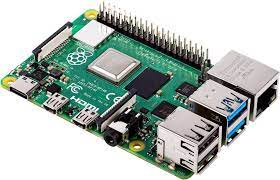
\includegraphics[width=4cm]{images/raspberrypi.jpeg}
\caption{Raspberry Pi}
\label{fig:raspberryPi}
\end{figure}

\subsection{\textbf{Raspberry Pi}}
% 사용자의 사진을 촬영하는 카메라를 통제하고 촬영한 사진을 웹서버와 통신이 가능하게 한다. 인공지능 모델이 사진을 기반으로 뇌졸중 여부를 판단한 결과를 다시 받아 다시 사용자에게 알려주는 역할을 맡았다. 이 과정은 NUGU 스피커로 청각적으로나 Dashboard를 통해 시각적으로 표현이 가능하다.
It controls a camera that captures user photos and enables communication with a web server. The artificial intelligence model is responsible for determining the presence of a stroke based on the photos and relaying the results back to the user. This process can be conveyed either audibly through NUGU speakers or visually through a dashboard. We use this to create a real IoT program.\\

\subsection{\textbf{SSH}}
To enhance coding productivity on Raspberry Pi, we use SSH. This allows us to remotely connect to the Raspberry Pi from our local desktop and use the same IDE for increased efficiency.
SSH enables the connection between the Raspberry Pi and the local desktop when they are on the same Wi-Fi network.\\

\subsection{\textbf{Camera}}
To execute our project, a camera is essential. Since we are planning to implement IoT technology using Raspberry Pi, we opted for the highly compatible camera, PiCamera2. This allows us to automatically forward the camera to camera-related functions used in OpenCV.\\

\subsection{\textbf{LED module}}
We use the LED module for privacy protection. When the device connects to the server or the internet, the LED lights up, allowing users to be aware of the current status. This is to prevent crimes resulting from hacking.\\

\subsection{\textbf{OpenCV}}

\begin{figure}[htp]
\centering

\includegraphics[width=2cm]{images/opencv.png}
\caption{OpenCV}
\label{fig:opencv}
\end{figure}

OpenCV is a powerful library widely used for computer vision and image processing tasks. It allows us to perform various operations, such as reading and saving images. Additionally, it provides the capability to perform color space transformations, which is crucial for efficiency. Resizing images is also possible, and OpenCV offers a wide range of algorithms and functions for tasks like face pattern detection. Furthermore, it allows for feature point extraction and image processing, making it a versatile tool for a variety of tasks.\\



\subsection{\textbf{Tensorflow Serving}}

\begin{figure}[htp]
\centering

\includegraphics[width=4cm]{images/tensorflow.png}
\caption{TensorFlow}
\label{fig:tensorflow}
\end{figure}

% Tensorflow를 기반으로 인공지능 모델을 개발했을 때, 배포를 간편하게 진행할 때 필요하다.
When developing an artificial intelligence model based on TensorFlow, it is necessary for streamlined deployment.\\

\subsection{\textbf{Privacy Protection}}
% 사용자의 사진을 촬영하는 카메라로서 사용되지 않는 경우에는 작동이 불가능해야 한다. 개인정보 보호를 위해 카메라가 작동 중이면 맥북의 웹캠처럼 표시를 가능하게 하거나 zoom의 기능과 같이 주변부를 흐리게 처리할 수 있다.
Privacy policy is of utmost importance in our project, given that it involves capturing a user's everyday life. We aim to ensure privacy through a two-step approach. \\
\subsubsection{\textbf{Background Blur}}
First, we will apply blurring to the background, excluding the face. \\
\subsubsection{\textbf{Two-level detection and LED module}}
Second, we will implement a real-time detection algorithm that operates locally without internet or server connectivity in normal circumstances. In the event of a detected risk of stroke, the system will establish a connection to the server, capturing an accurate photo of the user to utilize a trained artificial intelligence model. If connected to the server or the internet, an LED module located next to the camera will activate, allowing the user to visually confirm the device's status.\\

\subsection{\textbf{Speaker}}

% 인공지능 스피커로 본 프로젝트에서는 라즈베리 파이에서 전송된 뇌졸중 여부를 사용자에게 청각적으로 전달할 수 있다. 이 외에 사용자가 원할 때 촬영을 시작하도록 trigger를 인식할 수 있다.
Using a speaker gives the ability to audibly relay stroke information sent from the Raspberry Pi to the user. 

\subsection{\textbf{Dashboard}}
% 뇌졸중 여부를 시각적으로 표현해준다. 라즈베리 파이에서 전송된 뇌졸중 여부와 확률, chatGPT로 작성한 건강에 관련된 유용한 정보를 사용자에게 시각적으로 보여준다. 유용한 정보의 예시는 다음과 같다. 뇌졸중에 도움이 되는 음식이나 생활습관, 만약 발병한다면 어떻게 해야 하는지에 대한 정보가 포함된다.
It visually expresses whether you have a stroke or not. It displays stroke information and its probability sent from the Raspberry Pi, along with health-related useful information generated by ChatGPT, to the user. Examples of useful information include foods and lifestyle habits that can be beneficial in the event of a stroke, as well as guidance on what to do if a stroke occurs.\\
\subsubsection{\textbf{Probability of Stroke}}
% API를 통해 전송된 값에서 뇌졸중 여부의 확률값을 표현한다. 자동차의 속도 계기판을 모티브로 하여 사용자에게 직관적으로 확률을 전달한다.
It expresses the probability value of stroke from the value transmitted through the API. It transmits probabilities to users by using as a motif the speed dashboard of a car.\\
\subsubsection{\textbf{User's Image}}
% 사용자를 촬영한 사진을 보여준다. 이로써 사용자는 자신의 상태를 객관적으로 확인할 수 있으며 경각심을 일으킬 수 있다.
It displays the photo of the user, allowing the user to objectively assess their own condition and potentially raise awareness of their health.\\
\subsubsection{\textbf{Treatment Options}}
% 아래의 chatGPT를 통해 얻은 뇌졸중의 치료법을 보여주는 공간이다. 만약 사용자가 뇌졸중의 확률이 높을 경우에는 더욱 눈에 띄도록 표현할 수 있다.
It shows treatment options obtained using ChatGPT. If the user has a high probability of stroke, these treatment options can be highlighted in order to draw even more attention to the user.\\
\subsubsection{\textbf{Prevention and Information}}
% 아래의 chatGPT를 통해 얻은 뇌졸중의 예방법을 알려준다. 뇌졸중의 확률이 낮더라도 예방법을 사용자에게 알려주고, 만약 의심될 때는 어떻게 해야하는지 행동지침을 알린다. 이로써 능동적인 건강관리를 가능케 한다. 
It tells users how to prevent themselves of gettting a stroke obtained and this information is also obtained by using ChatGPT. Even if the probability of stroke is low, it still informs the user of preventions and informs him on the behavioral guidelines to have in suspicion of stroke. This enables daily active health care.\\

\subsection{\textbf{ChatGPT}}

\begin{figure}[htp]
\centering

\includegraphics[width=2cm]{images/chatgpt.png}
\caption{ChatGPT}
\label{fig:chatgpt}
\end{figure}

% 사용자의 뇌졸중 여부와 확률을 기반으로 유용한 정보를 생성해주는 생성형 AI이다. API를 이용해서 질문을 담아서 전송하고 답변을 다시 받아온다. 그 답변을 Dashboard 혹은 NUGU를 통해 사용자에게 알려준다. 
It is a generative AI that generates useful information based on the user's stroke status and probability. It uses API to send questions and receive answers. The answer is notified to the user through the Dashboard or the NUGU Speaker.\\
\subsubsection{\textbf{Question}}
% chatGPT에게 뇌졸중 관련으로 질문할 때 피상적인 표현으로 한다면 당장 병원에 가야한다는 정보만 얻는다. 인공지능 모델이 반환한 결괏값에서 확률을 추출하고 치료법과 예방법, 병원을 어떻게 골라야하는지를 직접적으로 물어본다. 
When asking questions related to strokes to ChatGPT, you only receive information suggesting an immediate need to go to the hospital. By extracting the probability from the results returned by the artificial intelligence model, we can inquire directly about treatment options, preventive measures, and guidance on selecting a hospital.\\
\subsubsection{\textbf{Answer}}
% 위의 질문 형식으로 chatGPT에게 질문하고 받은 대답이다. 이 대답은 Dashboard 혹은 NUGU로 전달되어 각각 시각적, 청각적인 표현으로 사용자에게 전달된다.
After using the question format above, the answer received from ChatGPT can be passed to the Dashboard or the NUGU Speaker then passed to the user in a visual or auditory representation.\\

\subsection{\textbf{Database}}
% 인공지능 모델의 정확도를 향상시키기 위해서 이미지를 보관하는 데이터베이스가 필요할 수 있다. 하지만 이는 개인정보로 민감할 수 있기에 데이터베이스 없이 프로젝트를 구현하는 것으로 진행할 수도 있다.
To enhance the accuracy of the artificial intelligence model, a database for storing images may be required. However, since this can involve sensitive personal information, the project can also be implemented without a database.\\